\documentclass[11pt,twocolumn]{MyTightStyle}
\usepackage{graphics}
\usepackage{url}
\usepackage{color}
\usepackage{epsfig}

\markboth{Draft - Do not redistribute}{Draft - Do not redistribute}
\newcommand{\fixme}[1]{{\color{red} #1}}
\newcommand{\comm}[2]{{\color{blue} (#1's comment: #2)}}
\newcommand{\eat}[1]{}

\usepackage[centertags]{amsmath}
\usepackage{amsthm}
\usepackage{epsfig}
\theoremstyle{plain}
\newtheorem{thm}{Theorem}
\newtheorem{cor}[thm]{Corollary}
\newtheorem{lem}[thm]{Lemma}
\newtheorem{prop}[thm]{Proposition}

\theoremstyle{definition}
\newtheorem{defn}{Definition}%[section]

\theoremstyle{remark}
\newtheorem{rem}{Remark}[section]

\numberwithin{equation}{section}
\renewcommand{\theequation}{\thesection.\arabic{equation}}



\begin{document}

\title{Verifiable Hierarchical Aggregation}

\author{
VeHAg Working Group
}

\maketitle

\begin{abstract}
\end{abstract}


\section{Introduction}
\label{sec:introduction}

Inspired by SIA~\cite{Przydatek2003}.

The purpose of this white paper is to codify existing or emerging
techniques for achieving verifiable data aggregation in the distributed
data model, when the aggregation function cannot be computed by a single
aggregator.



\section{Problem Setup}

There is a population $D$ of data sources and a population $A$ of
aggregators.  $A$ and $D$ are known (system-wide) and there exists a
public key infrastructure allowing all nodes in $D$ and $A$ to sign and
encrypt messages.

Data sources in $D$ emit values in $\{0, 1\}$.  We wish to supply a
querier $Q$ with the count of 1's emitted by the members of $D$ with
known error bounds and confidence intervals.
Aggregators in $A$ can assist $Q$ by performing intermediate
computations on data emitted by $D$.

Aggregators and data sources are organized in a directed acyclic graph
$G$ whose edges determine the transfer of a datum or intermediate
result.  Data sources have in-degree of 0.  Aggregators perform their
function on all values arriving at their in-edges and send our the
result on all out-edges.  The graph $G$ is known.

The execution model is equivalent to post-order depth-first traversal:
each aggregator receives all values from its children (aggregators or
data sources connected to its in-edges) before it computes its function
and forwards it to its ancestors (aggregators or querier connected to
its out-edges).  No network losses occur.



\section{Approaches}

We explore counting over a canonical tree with deep spot-checking,
duplicate-insensitive estimation of the count with multiple submissions
of the same value to the same tree, and duplicate-insensitive estimation
of the count with multiple submissions of the same value to multiple
trees.

\begin{figure*}
\begin{center}
\includegraphics{AdditionTree}
\caption{\label{fig:AdditionTree} Circles are aggregators, squares are
data sources.}
\end{center}
\end{figure*}

\subsection{Additive count over canonical tree}
\label{sec:additionOverTree}
Let $G$ be the topology produced by placing aggregators in a full
\emph{m-way} tree and linking $|D|/|A|$ data sources to each aggregator.
Figure~\ref{fig:AdditionTree} shows an instance of such a graph (3-way
aggregator tree with 4 data sources per aggregator).

Each aggregator sums the values received from its children (other
aggregators and data sources) and forwards the result to its parent in
the graph.
\begin{defn}
A \emph{correct} aggregator is one that:
\begin{enumerate}
  \item Sums correctly all received data source values.
  \item Sums correctly all children aggregators' values.
  \item Reports to its parent the true value it computed.
  \item Checks each reported value for proper magnitude, given its
  position in the graph. Since, there are a fixed number of aggregators
  in a given aggregator sub-tree, there is also an upper bound on the
  value reported by any aggregator node.  In
  Figure~\ref{fig:AdditionTree}, aggregator 2 reports to 1 with regards
  to a total of 4 aggregators or 16 data sources; as a result, its
  reported sum cannot be greater than 16.
\end{enumerate}
\end{defn}

Using the above correctness definition, we can design an interactive
test to verify fully the correctness of a given aggregation graph, one
aggregator at a time, starting with the root (e.g., in a depth-first
traversal).  For each aggregator, we ask for its inputs received (which
data source gave which value and which child aggregator gave which
partial result) and outputs produced.  Given this evidence, we can
perform magnitude tests on inputs, we can check the consistency of
outputs with inputs reported by ancestors, we can validate the
transformation from inputs to outputs (i.e., sumation), and we can
verify that the inputs and outputs are consistent with the topology
$G$.  In Figure~\ref{fig:AdditionTree}, to check aggregator 3 (after
having checked 1), we check that its output matches the input reported
by 1 as coming from 3, we check that inputs come from its four data
sources and 8, 9, and 10, we check that aggregator inputs have values in
$[0,4]$ whereas data source inputs have values in ${0,1}$, and check the
correctness of the sumation.

Verifying the entire aggregation tree offers a certain correctness
guarantee that is equivalent to performing the entire computation by the
querier.  To reduce the cost of the verification, the querier can apply
this verification procedure on a sample of all aggregators.

We propose verifying the aggregators on random paths from the root
aggregator to a leaf aggregator.  Starting with the root, we choose
uniformly at random one of its children aggregators and proceed to
verify that until we reach a leaf in the aggregation tree.  If we perform
multiple random walks, making independent random decisions, we obtain a
sampling mechanism that selects nodes on a given aggregator level
independently and with uniform probability. Therefore, performing
$1/\epsilon$ random root-to-leaf walks will ensure with probability at
least $1-1/e$ that at most $\epsilon$ fraction of all aggregator nodes
on a given tree level are incorrect (Appendix~\ref{sec:sampling}). We
can repeat the $1/\epsilon$ random walks $\ln(1/\delta)$ times to
achieve probability of at least $1-\delta$.

\subsubsection{Analysis}
\label{sec:additionOverTree:analysis}
In this section we analyze the security and correctness guarantees of
the aggregation procedure described in
Section~\ref{sec:additionOverTree}.


If we run $1/\epsilon\times\ln(1/\delta)$ random walks through the tree,
all encountering only correct aggregators, then we know the following:
\begin{itemize}
\item At level $l$ of the aggregator tree, there are no more than
  fraction $1/\epsilon$ incorrect aggregators with probability at least
  $1-\delta$ at level $l$.  This follows directly from sampling the
  aggregators at a single level; the sampling is uniform and random over
  the coin tosses used to pick an entry at that level.  An implication
  of this is that, over the entire tree, there are no more than fraction
  $1/\epsilon$ incorrect aggregators with probability at least
  $1-\delta$.
\item An incorrect aggregator that is $k$ levels from the fringe of the
  aggregator tree can report a count that is at most
  $\frac{|D|}{|A|}\frac{m^{k+1} - 1}{m - 1}$ off the correct value (see
  Lemma~\ref{lem:offset}).
\item At a tree level $k$ above the fringe of the tree, incorrect
  aggregators can offset the result by at most $\epsilon |D|$ with
  probability at least $1-\delta$ (see
  Theorem~\ref{thm:faulty}).
\end{itemize}


The aggregation tree is a full \emph{m-way} tree with a total of
$|A|$ nodes. Let $l$ be the height of the tree. We have:

\begin{eqnarray*}
a &=& m^0 + m^1 + \ldots + m^{l-1}\\
a &=& \frac{m^l -1}{m-1}\\
l &=& \log_m(am-a+1)
\end{eqnarray*}


\begin{lem}\label{lem:offset}
A faulty aggregator that is $k$ levels higher than a leaf node ($0 \leq k
\leq l-1$) can report an aggregation result that is at most 
$\frac{|D|}{|A|}\frac{m^{k+1} -1}{m-1}$ higher(lower) than the correct one.  
\end{lem}

\begin{proof}
A leaf node in the aggregation tree controls $n/a$ data values. Each
value can be ether 0 or 1. Therefore, each leaf aggregator can offset
the correct result by $\frac{|D|}{|A|} = \frac{|D|}{|A|}\frac{m^{0+1}-1}{m-1}$.
Let for some $p \geq 0$ we have that an aggregator node at a distance
$p$ levels from the leaves of the aggregation tree can offset the
result by at most $\frac{|D|}{|A|}\frac{m^{p+1}-1}{m-1}$. An aggregator
node, one tree level higher, receives data from $|D|/|A|$ data source
nodes, as well as $m$ aggregators from the lower level. Since, each of
the lower level aggregators can offset the result by at most
$\frac{|D|}{|A|}\frac{m^{p+1}-1}{m-1}$, we have that the higher level
aggregator can offset the result by at most:
\begin{eqnarray*}
m\frac{|D|}{|A|}\frac{m^{p+1}-1}{m-1} + \frac{|D|}{|A|} &=&
\frac{|D|}{|A|}\frac{m^{p+2}-m+m-1}{m-1}\\
&=& \frac{|D|}{|A|}\frac{m^{p+2}-1}{m-1}
\end{eqnarray*}
From the principle of induction it follows, that an aggregator $k$
levels higher than a leaf node in the aggregation tree can report an
aggregation result that is at most $\frac{|D|}{|A|}\frac{m^{k+1} -1}{m-1}$
higher(lower) than the correct one.
\end{proof}

\begin{thm} 
\label{thm:faulty}
If at most $\epsilon$ fraction ($0 \leq \epsilon \leq 1$)
  of the aggregators on a given aggregator tree level are faulty,
  cumulatively  they can offset the correct aggregation result by at
  most  $\epsilon |D|$.
\end{thm} 

\begin{proof}
Using our notation, we have that the aggregation tree is a
full \emph{m-way} tree with height $l$ and a total of $|A|$ tree nodes, where
$l = \log_m(|A|m-|A|+1)$. An aggregation tree level that is $k$ ($0 \leq
k \leq l-1$) levels higher than the leaf level, has $m^{l-1-k}$ nodes. We
have that at most $\epsilon$ fraction of them are faulty, giving us at
most $\epsilon m^{l-1-k}$ faulty nodes on the level. From
Lemma~\ref{lem:offset} we have that each of the faulty nodes can
offset the result by at most  $\frac{|D|}{|A|}\frac{m^{k+1} -1}{m-1}$. Let
$F$ be the cumulative error caused by all faulty nodes. We have
that:
\begin{eqnarray*}
F &\leq& \epsilon m^{l-1-k} \frac{|D|}{|A|}\frac{m^{k+1}-1}{m-1}=\\
&=& \epsilon \frac{|D|}{|A|}\frac{m^l}{m^{k+1}}\frac{m^{k+1}-1}{m-1}=\\
&=& \epsilon \frac{|D|}{|A|}\frac{|A|m-|A|+1}{m^{k+1}}\frac{m^{k+1}-1}{m-1}=\\
&=& \epsilon n\frac{|A|m^{k+2} - |A|m^{k+1} + m^{k+1} - |A|m + |A|
  -1}{|A|m^{k+2} - |A|m^{k+1}}=\\
&=& \epsilon |D| (1 + \frac{m^{k+1}-|A|m + a -1}{|A|m^{k+2} - |A|m^{k+1}})
\end{eqnarray*}
Let's examine the conditions under which the second summand
is at most zero:

\begin{eqnarray*}
&\frac{m^{k+1}-|A|m + |A| -1}{|A|m^{k+2} - |A|m^{k+1}} \leq 0 &\Leftrightarrow\\
\Leftrightarrow&m^{k+1}-|A|m + |A| -1 \leq 0&\\
\Leftrightarrow& |A|(m-1) \geq m^{k+1}-1&\\
\Leftrightarrow& |A| \geq \frac{m^{k+1}-1}{m-1}&
\end{eqnarray*}
But we also have that $0 \leq k \leq l-1$ and $|A| =
\frac{m^l-1}{m-1}$. Therefore, the above condition is true for all
valid values of $k$.

$\Rightarrow F \leq \epsilon |D|$.
\end{proof}



\begin{figure}
\begin{center}
\includegraphics{faultyTrees}
\caption{\label{fig:faultyTrees} The thick line represents the path of
  values upwards from the two colored incorrect aggregators to the root,
  where the effect of an incorrect aggregator will apply to the outcome
  of the aggregation.  An incorrect aggregator can misreport its own
  partial value by up to the sum of all data sources and aggregators
  under the subtree of which it is the root.  For the light gray
  aggregator, this is the ``area'' (in terms of data sources) in the
  light gray triangle. For the dark gray aggregator, this is the
  ``area'' in the dark gray triangle, including the light gray triangle.
  The error induced by the light gray triangle is only counted once.}
\end{center}
\end{figure}

We would like to know something about the total error that incorrect
aggregators over the entire tree can induce.  A straightforward
extension of Theorem~\ref{thm:faulty} to $l=\log_m(|A|m-|A|+1)$ levels
points to an overall error of no more than
$\mathcal{O}(|D|\epsilon\log(|A|))$. This seems to be a loose upper
bound, given that incorrect aggregators placed within the subtree of
another incorrect aggregator cannot add their error to that of their
incorrect ancestor (see Figure~\ref{fig:faultyTrees}).  Instead, we
would like to compute the maximum error induced only by incorrect
aggregators that have no incorrect ancestor in the aggregation tree.  In
Figure~\ref{fig:faultyTrees}, this is the area within the three
thick triangles.


XXXX The following looks wrong XXXX


\begin{thm} The hierarchical aggregation algorithm produces with
  probability at least $1-\delta$ a result
  that is within $\epsilon n$ from the correct result.
\end{thm}

\begin{proof}
Each incorrect node that is undetected after the sampling is the root
of a sub-tree, no node of which has been traversed during
selection. All faulty nodes in $T$ can be organized into a set of
subtrees $K = \{T_1, T_2,\ldots T_k\}$, so that the root of $T_i$ is
the incorrect node $n_i$ and all ancestors of $n_i$ are correct. Clearly all incorrect
nodes in $T$ fall in one of the $T_i$


Moreover, any node in $T_i$
can be incorrect: sampling did not visit the root of $T_i$. By
sampling the tree, we know that with probability at least $1-\delta$,
there are no more than $\epsilon a$ incorrect aggregator nodes.

$\Rightarrow \sum_{i=1}^{k}|T_i| \leq \epsilon a$ with probability at
least $1-\delta$. Since each of the
faulty aggregators controls $n/a$ data source values, the total error
will be at most $\epsilon a \times n/a = \epsilon n$, with probability
$1-\delta$.
\end{proof}






















\subsection{Probabilistic Counting over Canonical Tree}
\label{sec:probabilisticCounting}

In this section, we explore the use of probabilistic set size estimation
techniques, such as that introduced by Flajolet and
Martin~\cite{Flajolet1985}, to tackle the same hierarchical counting problem. The basic idea
is to inspect a set of random numbers as large as the set whose size we
wish to estimate, looking for bit patterns in the random numbers that
are increasingly likely as more of them are inspected.  The
Flajolet-Martin (FM)~\cite{Flajolet1985} scheme keeps track of the
lengths of same-bit prefixes in the random numbers inspected.
The first
such length that does not apply to any random number inspected (when all
shorter lengths have) must be 
proportional to the base-2 logarithm of the number of trials.

Intuitively, half of the
random numbers must have a 0 first bit, a quarter of them must start
with two 0 bits, an eighth must start with three 0 bits, etc.  If in the
end it is found that a random number was found that starts with $k-1$ 0
bits but no number starts with $k$ bits, then about $2^k$ random numbers
must have been inspected (within a constant multiplicative factor).
Other such probabilistic counting schemes look for the smallest random
number inspected, for the largest $k-th$ smallest random number, or
other patterns.  To track this information, only a small word (on the
order of the logarithm of the expected cardinality) is required,
although to increase accuracy, the algorithm must usually be applied
multiple times independently.  For
every random number inspected, the bit position of the first 1 bit of
the number is set in this word.  In the end, the position of the first 0
bit in the word is used to estimate the cardinality of the set.

In the context of our problem, we wish to estimate the size of the set
of all data sources submitting 1 answers (e.g., the set of their
identifiers).  To emulate a random number source, every responding data
source can apply a secure hash function to its identifier and take the
result as the random number to use with FM.

To facilitate with validation of partial results up the aggregator tree,
the unit of information flowing up the tree (for a single trial of the
algorithm) has the form \{$\mathit{FMVal}$, [$d_i$, $\mathit{sig}(q)$]
\}, where $\mathit{FMVal}$ is the FM bit string built so far during the
aggregation, and every 1 bit in this bit string has associated with it
a support pair [$d_i$, $\mathit{sig}(q)$].  This support pair contains
the identity of a data source $d_i$ that set that bit, and a signature
by that data source on the current query $q$.   
A verifier (e.g., the aggregator receiving this
message) accepts this partial result only if, for every position $x$ at
which the bit string has a 1 bit, the hash of the associated
data source identifier $h(d_i)$ has its first 1 bit in position $x$, and
$d_i$'s signature on the query identifier $q$ is valid.
To aggregate multiple partial results, an aggregator performs a bitwise
OR on all FM bit strings, and keeps one of perhaps multiple identities
supporting each 1 bit, discarding the rest.
In the worst case, a submission
flowing up the aggregation tree carries a logarithmic number of
signatures in the domain of set cardinalities.  See
Figure~\ref{fig:FMAggregation} for an example.

\begin{figure}
\begin{center}
\includegraphics{FMAggregation}
\caption{\label{fig:FMAggregation} Two submissions (at the bottom) are
  aggregated to produce the one at the top.  Each submission bit has a
  supporting signature and signer's identity hash ``hanging'' from it.
  For example, in the bottom left, the fourth bit from the right is set
  because data source $A$ wanted to submit a 1 and $h(A) = 11000$.  At
  the top for the same bit position, the aggregator could have chosen
  either $A$'s signature or $C$'s signature, but chose $A$'s.}
\end{center}
\end{figure}


\subsubsection{Analysis}
\label{sec:probabilisticCounting:analysis}

A verifier who receives the submission yielded by the root aggregator
can verify that all enclosed signatures support the contents of the
submission (as in fact all aggregators also do).  Since incorrect
aggregators cannot forge data sources' signatures on bit supports, no
malicious aggregator can ``create'' 1 bits in the aggregated bit string
that no data source supported.

However, a malicious aggregator may
have \emph{suppressed} 1 bits, replacing them with 0 bits for some bit
positions.  The only way for a verifier to validate a 0 in a bit
position is to ensure that \emph{no data source} had a submission
setting that bit position to 1.

The adversary can benefit from suppressing 1 bits in earlier positions
than the first 0 bit.  For example, in Figure~\ref{fig:FMAggregation},
the adversary would not benefit from suppressing the 1 in the 4th bit
positiong from the left, since there is a 0 bit in the 3rd position,
based on which FM will estimate the size of the set.  Suppressing the
1 in the 2nd bit position from the left would be more useful, since it
would effectively halve FM's estimate of the set size.  On the other
hand, if the figure depicts an intermediate stage in the aggregation,
suppressing the 4th bit position might prove useful if the 3rd bit
position is likely to be eventually set, closer to the aggregation root.

In general terms, the further to the left a 1 bit is, the less likely it
is to be set (the probability decreases exponentially with the bit
position), and the less dramatic its suppression will be on the result
of the estimate (which might also mean a less detectable suppression).

The positioning of incorrect aggregators in the aggregator tree is also
very important.  The closer to the root an aggregator is, the greater
opportunities it has to affect the final result.

We explore two primary approaches for reducing the ability of incorrect
aggregators to suppress 1 bits in this scheme: redundancy in trees and
redundancy in data submission.  Figure~\ref{fig:FMRedundancies}
illustrates the two.

\begin{figure}
\begin{center}
\includegraphics{FMRedundancies}
\caption{\label{fig:FMRedundancies} The figure shows two ways for a data
  source to submit its value redundantly.  On the left, it submits its
  value multiple times to the same tree but different leaf aggregators.
  On the right, it submits its value to multiple trees.}
\end{center}
\end{figure}


\subsubsection{Redundant Aggregation Trees}

If the FM aggregation scheme runs over multiple, randomly constructed
trees, then the benefit obtained by an incorrect aggregator placed high up in
one tree is offset by a high likelihood that the aggregator will be
placed lower in another tree.

Furthermore, a rare 1 bit that is successfully suppressed by an
incorrect aggregator in one tree is likely not to meet that aggregator
in another tree.

\subsubsection{Redundant Data Submission}

Maintaining multiple aggregation trees may be expensive.  An alternative
to running the FM aggregation scheme over multiple trees is running it
over the same aggregator tree, but with a different mapping from data
sources to leaf aggregators.


\subsubsection{Other Ideas}

It is possible to explicitly count 0 answers as well as 1 answers, by
repeating the FM scheme so as to probabilistically count the identities
of those submitting a 0.  This would take twice as much effort and
bandwidth, though the number of messages would arguably remain the
same.  

{\bf Count by Set Size Estimation: } Let's assume that we have an
algorithm $A$ that can estimate the size of a set with some customizable
precision.  How can we use this algorithm to estimate the result of a
COUNT() aggregation operation? For this purpose let us introduce some
notation. Let $X$ be the correct set of all data source values that have
a value of 1, $Y$ be the correct set of all data source values that have
a value of 0, and $Z = X \cup Y$ be the set of all data source
nodes. Let also $X'$ be the set of data source values that are claimed
to be 1, $Y'$ be the set of the datasource values that are claimed to be
0, and $Z' = X' \cup Y'$. Finally, we will use $\widetilde{X}$ to denote
the estimate of $X$ obtained by running the algorithm for set size
estimation.

\comm{A}{We assume that the data sources are correct. This means that
          when they receive a query they do send a corresponding
          value. The problem with using set size estimation directly is
          that even with perfect set size estimation, we do not know if
          all data sources have received the query. If we sample the
          data sources to see if they received the query, then we can
          ensure that no more than $\epsilon$ fraction of the data
          sources have not received the query. This will directly
          translate into getting a relative error in terms of the number
          of data sources, not the number of data sources matching the
          predicate. }

Clearly, if we have direct access to $X$, we can compute its size and
solve the problem. However,  in practice we have access to only $Z$, $X'$,
and $Y'$.

{\bf Solve the problem by using $Size(Z)$}\\
One can compute count using the following approach:
\begin{enumerate}
  \item Compute the size of $Z$
  \item Compute the size of $X'$
  \item Compute the size of $Y'$
\end{enumerate}

If we assume that there are no failures during the process, we can
expect that $Z = X' + Y'$.


We would like to use $X'$ to compute the aggregation result, but
we need to ensure that:

\begin{enumerate}
  \item $X'$ does not contain too many falsely claimed 0s.
  \item $X'$ does not exclude too many elements of $X$.
\end{enumerate}

We can ensure the first guarantee by sampling $X'$. We can examine at
random $1/\epsilon$ elements of $X'$ and ensure that they all have 1
values. This will guarantee that $X' \leq (1+\epsilon) X$ with probability
$1-1/e$. To satisfy the second requirement, though, we need to sample
elements from $X$. However we do not have access to $X$. We can sample
elements from $Z$ and stop after we collect the desired number of
samples from $X$. The number of elements of $X$ that we need to
examine before we obtain the desired sample is dependent on the
selectivity of the predicate ($0\leq s \leq 1$) and its expected value
is $\frac{1}{s\epsilon}$. For predicates with relatively low
selectivity this number can be significant.

We can avoid the need to sample from $X$ by using $Y'$ in the
computation of the aggregate. We can sample $Y'$ to ensure that $Y'
\leq (1+\epsilon)Y$. We can then sample from $Z$ and make sure that each
sampled element is in either $X'$ or in $Y'$. If we take $1/\epsilon$
samples we know that $X' + Y' \geq (1-\epsilon)(X+Y)$. We can continue
sampling until we collect $1/\epsilon$ samples from either $X$ or
$Y$. In the worst case this process will require at most $2/\epsilon
-1$ samples. If we were lucky to collect the samples from $X$, then we
have $X' \geq (1-\epsilon)X'$ and together with the earlier result of
$X' \leq (1+\epsilon) X$, we have that $(1-\epsilon)X \leq X'(1+\epsilon)X$. 

If we were unlucky and selected more elements from $Y$, then $Y' \geq
(1-\epsilon)Y$. We have that:
\begin{align*}
                  & X' + Y'  \geq (1-\epsilon)(X+Y)\\
  \Leftrightarrow & X'       \geq (1-\epsilon)(X+Y)-Y'\\
                  &          \geq (1-\epsilon)(X+Y)-(1+\epsilon)Y = (1-\epsilon)X -2\epsilon Y\\
  \Leftrightarrow & X'       \geq X -\epsilon(X+2Y)
\end{align*}

%$\Rightarrow (1-\epsilon)X \leq X' \leq (1+\epsilon)X$.




\bibliographystyle{plain}
\bibliography{vehag}













\appendices
\section{Sampling to estimate the size of a subset}
\label{sec:sampling}
Problem: Let $S$ be a set of $n$ elements. Each $s_i \in S$ belongs to
one of the two classes: ``Good'' or ``Bad''. To test the properties
of $S$, we take a random sample of size $m$. How big should $m$ be, so
that if all samples are ``Good,'' the fraction of 
``Good''  elements in $S$ is at least $(1-\epsilon)$ with
constant probability?

Solution: The probability of all $m$ sample elements being ``Good,'' while
there are at least $(1-\epsilon)n$ ``Bad'' elements is
$(1-\epsilon)^{m}$. We want to bind this number from above with the
constant probability $\delta$:
\begin{eqnarray*}
(1-\epsilon)^{m} \leq \delta &\Leftrightarrow& m\ln{(1-\epsilon)} \leq \ln{\delta}\\
&\Leftrightarrow& m \geq \frac{\ln{\delta}}{\ln{(1-\epsilon)}}
\end{eqnarray*}
Since $\ln{(1-x)} \leq -x$, we must also have
\begin{eqnarray*}
m \geq \frac{\ln{\delta}}{-\epsilon} = \frac{1}{\epsilon}\ln{(\frac{1}{\delta})}
\end{eqnarray*}

Thus by setting $m \geq \frac{1}{\epsilon}\ln{(\frac{1}{\delta})}$, we
satisfy the condition that with probability at least $(1-\delta)$, $S$
contains at least $(1-\epsilon)n$ ``Good'' elements.




\cleardoublepage 



\section{Result}

%\section{Correctness Definition}
%Let $\mathcal{D}$ be a collection of data sources and $\mathcal{A}$ be
%a population of aggregator nodes. Let $|\mathcal{D}|=d$,
%$|\mathcal{A}|=a$ ($ a \leq d$) , and $\mathcal{D} \cap \mathcal{S} =
%\emptyset$. 

%Different configurations are possible: $\mathcal{A} \subseteq
%\mathcal{D}$, $\mathcal{D} \cap \mathcal{A} = \emptyset$, or
%$\mathcal{D} \cap \mathcal{A} \neq \emptyset$. This is to say that
%some (all) aggregator nodes can also be data source nodes. Let
%$|\mathcal{D}\cup\mathcal{A}| = n$.

%Aggregator
%nodes are organized in some hierarchy that allows them to process data
%provided by the data sources. Data processing is distributed - data
%source nodes send data to aggregators and  aggregators perform local
%computation by applying a function $f()$ over all data they
%receive. The result of each local 
%computation is forwarded to other aggregator nodes, so that at the end
%of this process, one or more aggregator nodes contain a value, which
%is identical to the result of
%applying $f()$ to all data provided by the data source nodes.


%We are interested in evaluating $f() = COUNT(P)$, the number of data
%source nodes that have data matching the given predicate $P$. We can
%compute this number by setting $f() = \sum_{all inputs}$, and limiting
%the range of the value provided by each data source node: $d_i \in
%\{0,1\}$. Because of the magnitude of $d$, it is impossible
%(undesirable) to send all data generated by the data sources to each
%aggregator. Because of the scale of the system, it is also impossible
%to verify the correctness of the processing performed by each
%aggregator. At the very best, we can afford to verify the operation
%of a constant number or a small fraction of aggregators.  

%Let $S = \sum_{i=1}^{d}d_i$ be the correct sum of all values reported
%by the data source nodes, and $\widehat{S}$ be the estimated sum using the
%hierarchy of aggregators. We define $r = |S-\widehat{S}|$ to be the
%absolute additive aggregation error, and $s = \frac{|bad
%  aggregators|}{a}$ - the subversion fraction.


%If we can tolerate at most $\epsilon$ fraction of all aggregator nodes
%to be faulty, i.e. to perform their aggregation operations incorrectly,
%then ideally we would like them not to be able to offset the final
%result by more than the fraction of the data that they control,
%namely: $\epsilon \times a \times \frac{d}{a} = \epsilon d$.
 

%-- want a distributed solution: spread work
%-- want correct result
%-- but do not trust individual aggregators
%-- trust data source nodes
%-- can inspect some aggregators and verify they are work
%-- cannot inspect all
%-- what is the quality of the end result


%Choose an aggregation hierarachy that imposes strong probabilistic
%bounds on the resulting relative error.

\subsection{Building Blocks}

\subsubsection{Mapping Values to Keys in a DHT}
\label{sec:mapping}

Without lack of generality, let's assume that the key space of a DHT
is a ring of size $K$. Let $V$ be a set of $n$ different values that
we want to map to DHT keys. The probability of assigning any $v \in
V$ to a given DHT key is uniform (making the necessary assumptions of
the hash function used). Let $A$ be the event of a DHT key not being
assigned to a value after $n$ consecutive assignments. We have that
$P(A) = (1- \frac{1}{K})^n$.

Let's partition the key ring into $a > 0$ equal size ranges. Let
$B$ be the event that a range constructed in this way is empty,
i.e. it contains no key that is mapped to any $v \in V$. The size of
each range is $\frac{K}{a}$. Therefore:

\begin{eqnarray*}
P(B) = ((1-\frac{1}{K})^n)^{\frac{K}{a}} =
(1-\frac{1}{K})^\frac{Kn}{a} \leq e^{-\frac{|D|}{|A|}}
\end{eqnarray*}

Let $E[B]$ be the expected number of empty ranges. We have that:
\begin{eqnarray*}
E[B] = a(1-\frac{1}{K})^\frac{Kn}{a} \leq ae^{-\frac{|D|}{|A|}}
\end{eqnarray*}   

Let $C$ be the event that a given range has exactly $n/a$ keys. We
have:
\begin{eqnarray*}
P(C) &=& {{\frac{K}{a}} \choose
  {\frac{|D|}{|A|}}}
  ((1-\frac{1}{K})^\frac{Kn}{a})^\frac{K-n}{a}(1-(1-\frac{1}{K})^\frac{Kn}{a})^\frac{|D|}{|A|}\\
&=&  {{\frac{K}{a}} \choose
  {\frac{|D|}{|A|}}}(1-\frac{1}{K})^\frac{Kn(K-n)}{a^2}(1-(1-\frac{1}{K})^\frac{Kn}{a})^\frac{|D|}{|A|}
\end{eqnarray*}


Let $X$ be a random variable describing the number of keys in a given
range that are mapped to some values in $V$. $X$ has binomial
distribution:
\begin{eqnarray*}
P[X=i] = {\frac{K}{a} \choose i}p^iq^{\frac{K}{a}-i}
\end{eqnarray*}
where $q = (1-\frac{1}{K})^n$ and $p=1-q$.

For the expectation of $X$ we have:
\begin{eqnarray*}
E[X] &=& \frac{K}{a}p = \frac{K}{a}(1-(1-\frac{1}{K}^n) =\\
&=& \frac{K}{a}(\frac{1}{K}(1+(1-\frac{1}{K}) + (1-\frac{1}{K})^2 +
\ldots + (1-\frac{1}{K})^{n-1})=\\
&=& \frac{(1+(1-\frac{1}{K}) + (1-\frac{1}{K})^2 +
\ldots + (1-\frac{1}{K})^{n-1})}{a}
\end{eqnarray*}

A typical value of $K$ is $2^{160}$ for which $\frac{1}{K} \approx 0$
and $E[X] = \frac{|D|}{|A|}$.

For the variance of X we have:
\begin{eqnarray*}
Var[X] &=& \frac{K}{a}pq = \frac{K}{a}\frac{(K-1)^n}{K^n}\frac{K^n -
  (K-1)^n}{K^n} =\\
&=& \frac{K(K-1)^n}{aK^n}\frac{K^{n-1} + K^{n-2}(K-1) + \ldots +
  (K-1)^{n-1}}{K^n} \leq \\
&\leq& \frac{K(K-1)^nnK^{n-1}}{aK^{2n}} = \frac{|D|}{|A|}(\frac{K-1}{K})^n
  \leq \frac{|D|}{|A|}
\end{eqnarray*}


\subsubsection{Selecting a Sub-set of Application Hosts}
\label{sec:selecting}
{\bf Problem:} Given a set of $n$ application hosts organized in a DHT
circular key-space of size K, choose with high probability a sub-set
of different application host of size $\frac{m^k-1}{m-1}$, where $k$
is maximal.\\

\noindent {\bf Solution:} To select $p$ (not necessary different)
application  hosts we can use the following algorithm. Split the
key-space into $p$ equal size ranges. For each range select the node
successor(beginning of range). The advantage of this scheme is that it
is efficient and convenient: to access the $i^{th}$ selected host, simply
compute successor(start of $i^{th}$ range). However, it is possible to
obtain less than $p$ different physical hosts, since some ranges can
be empty. In Section~\ref{sec:mapping} we calculated the probability
of a single range being empty to be at most $e^{-\frac{n}{p}}$ and
the expected number of empty ranges to be at most
$pe^{-\frac{n}{p}}$. Therefore, to solve the problem, we can use the
simple selection mechanism with the largest value of $p$ for which the
expected number of empty ranges becomes close to zero. This procedure
will give us with high probability $p$ different application hosts.

\subsubsection{Estimating the Number of Application Hosts}
\label{sec:estimating}
{\bf Problem:} Let there be $n$ application hosts organized uniformly in a
circular key-space. Devise an algorithm to estimate $n$, with limited
communication and computation.

\noindent {\bf Solution:} Let the key-space be of size $K$. Let $X$ be
a random variable equal to the distance (in key-space) between two
consecutive application hosts. We can estimate $E[X]$ by using the
observation that the $n$ nodes partition the key-space in $n$ disjoint
intervals, the sum of which is $K$. Therefore the average interval
size is: $E[X] = \frac{K}{n}$. Therefore, given $E[X]$, we have $n =
\frac{K}{E[X]}$.

We can approximate $E[X]$ by using sampling. Let $\overline{X}$ be the
mean of the observed $m$ samples. We know that $E[\overline{X}] = E[X]$
and $Var[\overline{X}] = \frac{Var[X]}{m}$. (Need to compute
$Var[X]$). From the Central Limit Theorem, we have that $\overline{X}$
is normally distributed. Therefore, $|X-\overline{X}| \leq
\Phi(t)\sqrt{\frac{Var[X]}{m}}$ with probability $t$, where $\Phi(t)$
is the abscissa of the vertical line, which cuts an area of size
$\frac{1-t}{2}$ from the unit normal curve. If $\widehat{n}$ is the
estimated value of $n$ using a sample of size $m$, we have with
probability $t$ that:
\begin{eqnarray*}
\frac{K}{\frac{K}{n} + \Phi(t)\sqrt{\frac{Var[X]}{m}}} \leq \widehat{n} \leq
  \frac{K}{\frac{K}{n} - \Phi(t)\sqrt{\frac{Var[X]}{m}} }
\end{eqnarray*}


\subsubsection{Building a Multicast Tree}
\label{sec:building}
{\bf Problem:} Build a spanning tree of degree $m$ of all application
hosts registered in a circular key-space.\\

\noindent {\bf Solution:} Let $v$ be the root of the spanning
tree. We define the visited list $L$ as the list of all nodes along a path
of the spanning tree visited by going top-down from the root. The root
of the tree adds itself to the visited list and partitions the key space
into $m$ equal size key 
ranges. For each key range it computes $v_i =
successor(beginning of range)$. If $v_i \notin V$, $v$ forwards the
visited list to $v_i$. Upon receiving the message, $v_i$ adds itself
to the visited list, calculates the boundaries of its range, splits it
into $m$ equal sizes, finds the successors of the beginning of
each sub-interval, and forwards the visited list to the successors not
yet in it. Using this recursive scheme the process terminates when all
application hosts have been visited. Using the uniformity assumption,
we can show that the average distance from the root to a leaf in the
tree is $\log_m(n)$, where $n$ is the number of application hosts. The
variance of this estimate is within small bounds (need to quantify it).



\subsubsection{Estimating the Cardinality of a Set}
Flajolet and Martin propose an algorithm to estimate the cardinality
of a set with customizable precision. The core idea of the algorithm
is to use randomization: each distinct element can contribute in a
deterministic way and the rate of the contribution can be exploited to
compute the cardinality of the set. A very useful property of the
algorithm is that it is insensitive to the underlying
distribution, as well as to repetition and multiple counting.

The algorithm works as follows. Let $B$ be a bitvector of size $r$, so that $r
> \log_{2}{n}$, where $n$ is the maximal possible cardinality, and let
$H$ be a hash function defined on the domain of possible set elements
with range $[0, 2^r-1]$. Define $\rho(\alpha)$ to be the position of
the left-most 1 bit in the binary representation of $\alpha$. For each
set element $x$, compute $\rho(H(x))$ and set the corresponding bit of
$B$ to 1. Using this approach on the average every second element sets
the bit at position 0, every fourth - the bit at position 1, etc. We
can compute the cardinality of the set as two to the power the position of the
left-most consecutive 1 bit. Flajolet and Martin derive more precise
formulas for the final conversion that correct also for the small
incurred bias.

It is possible to improve the standard error of the above aproach by
repeating it multiple times and taking the average result. Flajolet
and Martin show that 64 repetitions result in precision of
approximately 10\%.

Mayank Bawa presented a small modification to the above
algorithm. Bawa's proposes to use coin flipping to compute $\rho$. For
each element key flipping coins intil the first time the flip results
in heads and use the trial number to mark the corresponding bit in 1. 

The Flajolet Martin algorithm gives in naturally to distributed
computation: if $B_1$ and $B_2$ are the bitvectors obtained by running
the algorithm on set $A_1$ and $A_2$ respectively, than the
cardinality of $A_1 \cup A_2$ can be determined from $B = B_1$ OR
$B_2$. 

\subsubsection{Estimating the Sum of a Set}
It is possible to estimate the sum of set by using the techniques for
set size estimation: transform the original set to a set, the
cardinality of which equals the sum of all set elements. Another
approach is to use repeated coin flipping as if each element consists
of a number of virtual elements equal to the magintude of its value.

Instead of flipping a coing multiple times, it is possible to flip a
biased coin and achieve the same result. Bawa describes the desired
biased coin probabilities.


\subsubsection{Sampling from a Tree}
Let $S$ be a set of data organized hierarchically in an m-way
tree. For simplicity let us assume that the set elements are stored at
the leaves of the tree and the internal tree nodes are simply used for
navigation. In many scenarios it is necessary to be able to obtain a
random uniform sample from $S$. If the underlying tree is a full tree
of $k$ levels, then any random root-to-leaf walk will generate a
random sample of a leaf node. However, if the tree is not full, some
walks will be shorter than others and as a result the probability of
visiting a leaf node will not be uniform.

To sample from a tree, we need to ensure that all walks give paths of
equal length. This means that the underlying tree has to be a full
m-way tree of maximal height. We can construct such a tree by placing
more than one element in a tree leaf. For an m-way tree, we can store
up to m elements in each tree leaf. If we use this organization, each
root-to-leaf walk will visit leaf nodes with uniform probability. To
ensure that all elements are visited with the same probability, we
need to inspect every single element stored in a given tree leaf.


It is interesting whether we can ensure that the tree structure is
maintained correctly by an untrusted entitity. We can define the tree
stucture more strictly as follows:
\begin{enumerate}
  \item All tree leaves are at the same level
  \item Each tree leave stores up to m elements
  \item If there are a total of $n$ leaves, all leaves up to $l_k$ ($0
  \leq k < n$) store $m$ elements, at most one stores more than 1 and
  less them m, and the remaining leaves store exactly 1.
\end{enumerate}

When we take a random walk, we can examine the path length of each
walk and the number of elements in each leaf. When we inspect we make
sure that:

\begin{enumerate}
  \item All path lengths are the same
  \item The three path is in sorted-order
  \item If two leaves, have different number of elements,  then they
  are at the correct location
  \item (when m> 2, at most one has more than 1 and less than m
  elements)
\end{enumerate}

If we take $1/\epsilon$ walks and ensure that they all stop on level
$l$ of the tree, what can we say about the tree?

The tree has $m^l$ nodes on level $l$. Let $n$ be the total number of
leaves in the tree. We have that at most $\epsilon m^l$ of the nodes
on level $l$ are not leaves: either lead to a leaf at a lower level or are the
continuation of a path that finishes at a leaf on a higher level.

$\Rightarrow n > (1-\epsilon)m^l$.

The problem here is that there can be a small number of heavy
sub-trees rooted at level $l$ and as a result the probability of
visiting a leaf in the heavy sub-tree is much smaller. To accomodate
for this the data structure maintainer needs to provide the upper
bound explicitly.

Tree commitment schemes using Merkle trees maintained by the prover
cannot be used to sample with uniform probability even if we try to
impose some predefined tree structure: we cannot impose an upper bound on the
number of nodes in the tree: the bound will have to be provided by the
prover.

Another problem with trees for sampling is repeating elements? 



note: there are two questions here: I commit to this set of data and
cannot add/remove any item at a later time. But i need not commit to
all. So if we want to make sure that i commit to all, we need some
oracle access to all.






\subsection{???}

\subsubsection{The Basics}
All application hosts are running on top of a Distributed Hash Table
(DHT). We make use of a publicly available DHT managed by a single
trusted authority. Clients of the DHT can install application code
in any DHT node and make use of the DHT public API. The main
characteristic of our platform is that application code has no access to
the DHT code and as a result cannot influence the correctness of the
DHT primitives. Therefore, in our work we assume that the DHT API are
trusted and hence always correct. However, application code is
vulnerable and is untrusted to perform its operations
correctly. Finally, there can be multiple applications running on
each DHT node, and not all DHT nodes are required to run the
same set of applications.

The DHT provides two basic primitives. The {\tt get(key)} primitive
retrieves the value stored under the specified key, and the
{\tt put(key,value)} primitive allows a client to store data under a
given key. There are two basic modes of servicing {\tt put()}
requests. In the \emph{overwrite} mode the new value overwrites any 
existing data stored under the key. In the \emph{append} mode values
are added to the already existing data. The DHT annotates each
stored value with the mode used in the corresponding {\tt put()}
operation.

\subsubsection{Application Hosts Registration}
All application hosts register themselves as members of the
application. Since the main target of our work is applications with
large number of hosts, centralized and broadcast registration are not
viable options. Our system requires a distributed membership
management scheme with provable correctness: if a malicious
application host decides to remove some other application hosts from
the system, it should be possible to detect this with high
probability. 

The ReDir protocol, provides a distributed membership management
mechanism. (Describe ReDir). 

A malicious host that uses the ReDir protocol, can remove
already registered application hosts by using put() in overwrite
mode. However, we can always detect this action by examining a given key
and inspecting the DHT annotations for each value. Should there be a
value with overwrite annotation, there has been some potentially
malicious action. While we can always detect malicious actions,
currently we have no mechanism to avoid them.

Another problem associated with the ReDir protocol is the ability of
an application node to put any identity during the registration phase. A
malicious host can put an identity under the wrong key, or can simply
insert an invalid identity. We can easily prevent against the first
threat by verifying that each identity we use falls in the current
range. The second threat, though, can cause significant problems
because it makes Sybil attacks possible: a single application host can
forge multiple identities and concentrate them in a single range of
the key-space, thus violating the uniformity of key
distribution. Uniform key distribution is important for the
performance and load balancing of our system.

To protect against Sybil attacks it is necessary to verify the
identity that an application host uses during ReDir registration. We
introduce a new put mode that treats the value parameter of the
put operation as the IP address of the client performing the
operation. To verify this IP address, the DHT establishes a handshake
with the client to protect against clients using spoofed IP
addresses. Other verification mechanisms based on public certificates
are also possible. 

Using the additional put mode, we can ensure that an attacker cannot
concentrate its presence in a given range of the key space and violate
the uniformity of key distribution. 

\subsubsection{Asking a Query}
We currently support queries counting
how many application hosts have data matching a given
predicate. We can support any general predicate that can be
applied to the data stored at each application host. When asking the
query, the client specifies the following parameters:
\begin{enumerate}
\item {\bf P} - the predicate to be execute at each data source node
\item {\bf s} - a random number uniformly chosen in the interval
  $[0,2^{160}-1]$ 
\item {\bf m} - the degree of the aggregation tree
\item {\bf a} - the number of aggregators to use in the evaluation of
  the query result
\end{enumerate}

To make query evaluation more resilient to long-term adversary attacks,
it is important to introduce variability in the aggregation hierarchy
used to evaluate the query. With static hierarchy, a long term
adversary can continuously corrupt aggregator nodes and obtain
significant presence. We introduce non-deterministic variability in
the aggregation hierarchy by using a random seed to determine its
root. 

The degree of the aggregation tree determines the amount of work
performed by each aggregator node, as well as the amount of work
performed in the query result verification phase. Larger values of $m$
translate into more work for each aggregator and more work to verify
the correctness of an individual aggregator. At the same time larger
values of $m$ translate into smaller tree height. (This is not
necessary the case, as depending on the value of $m$, we might
actually choose more aggregators).

Estimating the number of aggregator nodes to use has the goal of
choosing an optimal aggregation tree size that will balance the work
evenly among all involved aggregator nodes. The higher the number of
the aggregator nodes, the smaller is the average number of application
data that they receive, and consequently the smaller the cost of
auditing a single aggregator node. Therefore, we want to chose the
largest possible number of aggregators so that the 
amount of work performed during the result verification phase is as small
as possible. However to choose an acceptable number of aggregators it
is necessary to have an estimate of the number of application hosts. 

There are various ways to obtain the number of application
hosts. Centralized solutions can give very accurate estimates but are
too costly for networks of large sizes. Having each node maintain a
membership information about all application hosts is another
alternative with the same problems. For applications with large number
of hosts, we need a lightweight approach to estimate the network size
with as high accuracy as possible. 

Viceroy described a mechanism to estimate $n$, by using the distance
(in key-space) between two consecutive hosts. In
Section~\ref{sec:estimating} we present the approach together with
some error bounds. Viceroy also concluded that taking a sample of size
at least $\log(n)$ gives asymptotically tight results. Symphony also
uses the same mechanism, but their simulations show that even a sample
of size 3 gives reasonable results (for their particular application).

Using the estimate for $n$ we can use the approach described in
Section~\ref{sec:selecting} to choose a maximal set of
aggregators. The query initiator does not perform the actual selection
-- she simply determines the values of $a$ and $m$, which together
with the random seed $s$, completely define the aggregation hierarchy.

Having gathered all necessary query parameters, the query initiator
selects a random application host and sends the query to this host. To
select a random application host, the query initiator chooses
uniformly at random a number $x$ in the range of the key-space, and uses
the ReDir protocol to discover the node $v=successor(x)$.   

\subsubsection{Query Dissemination}
When an application host receives a query from a query
initiator, it initiates the process of query dissemination. Ideally,
we would like application hosts to receive the query, so that the
final result can be an accurate representation of the data in the
whole system. Alternatively, we can combine a best effort
dissemination approach with sampling to ensure that no more than
$\epsilon$ fraction of the application hosts have not received the
query. The 
advantage of sampling  is that we can use any best effort
approach to send the query and still get a good guarantee of the
correctness of the dissemination process. If sampling is successful, then
probabilistically the query dissemination has succeeded. A
disadvantage of this approach is its probabilistic nature, the
possibility of $\epsilon$ fraction of the application hosts being
unaware of the query, and the susceptibility to denial of service
attacks.

To disseminate the query we can use any existing multicast mechanism
such as Scribe, ReDir, or the simple scheme presented in
Section~\ref{sec:building}. 


\subsubsection{Aggregation Tree Construction}
We construct the aggregation tree using the simple selection mechanism
described in Section~\ref{sec:selecting} with the requirement that the
first key range starts at the random seed given in the query.

Each application host determines in which part of the key space it is
located by using its own identifier and the random seed $s$. Having
done this it sends a message to the successor of the beginning of its
range. The message contains the result of executing the predicate (0
or 1) and the hash of the query all signed with the key of the host. If
the node is not the successor of the beginning of its range, its part
of the process is over. If the node is the successor of the beginning
of its range, it starts a timer within the expiry of which it  has to
receive data from its children that are not aggregator nodes. Having
received the data, it verifies that they indeed are part of its range
and computes the sum. 

If the node is a leaf in the
aggregation tree (can be determined by the index of its range), then
it simply forwards the result with the hash of the query (digitally
signed) to its parent (can also be determined from the index of the
nodes' range). If the node is an internal node of the aggregation
hierarchy, it starts another timer and waits for its child aggregator
nodes to report their values. The duration of this timer depends on
the height of the tree and is proportional to the number of nodes in
the aggregator's sub-tree. Once all aggregator children report their
value, the node sums the values, adds the sum of the values of the
hosts in its range and forwards the result to its parent. 

\subsection{Verification}
The goal of query verification is to establish probabilistic bounds on
the quality of the aggregation result. Using verification we want to
ensure that the dissemination phase of query execution has reached at
least $(1-\epsilon)$ fraction of all application hosts. This is an
important requirement since it guarantees that the end result is
computed over a substantial number of the system hosts. The second
goal of verification is to ensure that at most $\epsilon$ fraction of
all nodes on each aggregation tree level are incorrect. We know from
Section~\ref{sec:additionOverTree:analysis} that this assurance translates into the
final result being off from the correct one by at most $\epsilon n$. 

We outline some modifications to the verification procedure outlined
in Section~\ref{sec:additionOverTree}. The need for modification arises
from the fact that unlike the situation described in
Section~\ref{sec:additionOverTree} in the P2P setting some aggregators will
receive data from more than $n/a$ hosts in their range, while others will
receive from less. In Section~\ref{sec:mapping} we estimated the
variance of the number of received values to be at most
$\frac{|D|}{|A|}$. This observation makes it possible for an aggregator
node to omit the value reported by a system host and we need a mechanism
to verify probabilistically whether there are more than $\epsilon$
fraction of omitted nodes. We can treat these omitted nodes as nodes
who did not receive the query.

We can inspect for omitted values by adding an additional verification
procedure. While inspecting an aggregator, choose uniformly at random
an application host that falls within its interval, and make sure that
its value is included. Using this technique, we can guarantee that at
most $\epsilon$ fraction of all application hosts that fall on a given
aggregation tree level have not received the query (and have not been
included in the result). Summing across all levels, we obtain the
required guarantee that at most $\epsilon$ fraction of all application
hosts have not received the query (not been included in the result). 


%NOTE: Somewhere we have to say something about virtual-physical
%nodes. The fact that more than one virtual nodes can be mapped to one
%physical node does not affect the correctness of the solution but
%affects the load distribution.





\subsection{Design Space}

(Mothy's Suggestion)

\begin{table}[htpb!]
  \centerline{
  \begin{tabular}{|c|c|c|}
    \hline
    Data Sources & Aggregators & Routers \\
    \hline
    T & T & T\\
    \hline
    U & * & *\\
    \hline
    T & T & U\\
    \hline
    T & U & U\\
    \hline
    T & U & T\\
    \hline
  \end{tabular}}
  \caption{\label{tab:scenarios} Possible Trust Scenarious}
\end{table}
  
We can describe the potential trust scenarious using
Table~\ref{tab:scenarios}. The system in question consists of three
main components. Data Sources provide data, Aggregators perform
computation over the data, and Routers supply aggregators with
data. Each of the system participants can be trusted (T) or untrusted
(U). Traditionally various research projects have studied the scenario
in which all system participants are trusted (row 1). These projects
have laid the foundation for out work. However, many realistic
scenarios not all system components can be trusted to perform their
operations correctly.

On one extreme of the possible spectrum are environments in which the
data source nodes cannot be trusted to provide correct data. This is
an extremely serious problem, because no matter whether the rest of
the system components are trusted or not, it is impossible to ensure
any correctness of the end result. This situation can be improved if
there exist mechanisms to verify the correctness of individual data
sources. However such mechanisms need to make use of historic
information and internal state transitions. Trust but Verify~\cite{}
is a project aimed at solving this particular part of
problem.

Moving further, we have three different scenarios which have not been
addressed so far. Our work focuses on the scenario corresponding to
the last row of the table. 
  

(Our Classification)
\begin{table}[htpb!]
  \begin{tabular}{|c|c|c|c|}
    \hline
    & No Trust & Trust but Verify & Full Trust\\
    \hline
    Querier Computes & Q1 & Q2 & Q3\\
    Network Computes & N1 & N2 & N3\\
    \hline
  \end{tabular}
\end{table}

There are two main approaches to compute an aggregate---have the
querier perform all computation (first table row), or have the network do
all computation. There are three main trust categories. No trust
describes situations in which no party is trusted to perform any
computation correctly, Trust but Verify describes situation in which
actors can be trusted but their work is subject to verification, and
full trust describes scenarios in which everyone is trusted to perform
computations correctly.

Querier Computation Based Solutions:\\
Solutions in this part of the design space have the querier to be the
only entity performing computation over all (some) of the data. There
are two main approaches in this class: make use of all data (provides
an absolute result), or utilize only a sample of the data (provides
relative result). Each of the two approaches is associated with
different cost and the sampling one is generally less expensive, but
also less accurate. There are different mechanism to collect the data
to be used in the computation. In the No Trust region (Q1) the
querier personally fetches the desired data, while in Q2 the querierier
specifies the desired size of the data and verifies that the delivered
data satisfies its requirements. 


Network Computation Based Solutions:\\
Solutions in this part do not involve the querier in the computational
process. In the No-Trust scenario, the querier uses redundancy to
obtain higher confidence about the correctness of the result that the
network provides. Redundancy can be expressed as either running the
same algorithm multiple times, or trying different algorithms. Of
particular interest is the last design space region N2. Solutions in
this region have the network compute the desired aggregation but
involve some kind of protocol in which the querier verifies the result
and asserts its correctness. 


Solutions by range and their results:

\begin{enumerate}
  \item [Q1] Querier Computes all, No Trust
    \begin{enumerate}
      \item Establish a connection with each data source, obtain its
      data, compute the result. Messages: $O(n)$, Computation: $O(n)$.
      
      \item Establish a connection with a predermined number of
      randomly chosen data source nodes. Extrapolate the result from
      the observed values: $O(sample size)$, Computation: $O(sample size)$.
      
    \end{enumerate}
  \item [Q2] Querier Computes all, Trust but Verify
    \begin{enumerate}
      
      \item The network collects all data and delivers it to the
      querier.

    \item The network collects a random sample and delivers it to
      the querier
    \end{enumerate}
  \item [N1] Network computes all, No Trust
    \begin{enumerate}
      \item Run the same algorithm multiple times and compare results
      \item Run different algorithms and compare results
    \end{enumerate}
  \item [N2] Network Computes all, Trust but Verify
    \begin{enumerate}
      \item Single Tree Aggregation with summing and sampling
      \item Single Tree Aggregation with modified Flajolet Martin
        and Sampling
      \item Multiple trees with no overlap
      \item Multiple trees with overlap
      \item Itermediary verification
    \end{enumerate}  
\end{enumerate}


Techniques:
\begin{enumerate}
  \item Redundancy
  \item Spot Checking
  \item Data Authentication
  \item Intermediate verification
  \item Different Heuristics
\end{enumerate}


\subsection{Butterfly Aggregation Hierarchy}
Instead of using a single aggregation hierarchy, it is possible to use
multiple hierarchies and redundancy to improve the quality and
reliability of aggregation. Let $a=m^l$. We can construct an m-way
Butterfly network by placing all aggregator nodes at each level of the network
and connecting each node on a given level to $m$ nodes on the level above
it, such that one of the nodes is the same node, and the other $m-1$
nodes are at specific distance, depending on the Butterfly level. Let
the bottommost Butterfly level be level 0. For $m^l$ nodes on 
every level, we have a Butterfly of a total of $l+1$ levels. 

We can perform aggregation using the Butterfly network. At level 0,
each aggregator node receives $n/a$ values from the corresponding data
sources and computes their sum. Having computed the sum, the
aggregator sends the result to the aggregator nodes on level 1 that it
is connected to. An aggregator at level 1, waits for its inputs to
arrive, computes their sum and forwards them to the next level. 

\begin{lem} If all aggregations have been performed correctly, the
  values reported by the butterfly nodes on the last level are the
  same and are equal to the total sum of all data source nodes.
\end{lem}

\begin{proof}
  An aggregator at level 0 computes the count of $d/a$ distinct data source
  nodes. An aggregator at level 1 receives data from  $m-1$ level 0
  aggregations to compute a sum over $mn/a$ distinct data source
  nodes. In the same way the aggregators on the last level ($l$)
  compute a sum over $m^ln/a = an/a = n$ distinct data source nodes.
\end{proof}


\begin{defn}
{\it Safe Cheating} - malicious actions of a single aggregator nodes
that affect in the same way the final values of all nodes at the
last Butterfly level. Safe cheating is indistinguishable be inspecting
only the values produced at the last Butterfly level.
\end{defn}

\begin{lem}
The result reported by an aggregator at level $i$ of the Butterfly
affects the outputs of $m^{l-i}$ aggregator nodes on the last
Butterfly level.
\end{lem}

\begin{proof}
At level $0$ we can reach any node on the last Butterfly level. This
follows from the construction of the Butterfly network - at each level
we shorten the distance by $1/m$ and in $l = \log_m{a}$ steps we can
reach the desired destination. Using the same reasoning, once we
are on level $1$, we have access to only $1/m$ fraction of the nodes
on the last Butterfly level. Using induction we can prove the claim of
the lemma.
\end{proof}

\begin{cor}
Cheating on level 0 is safe
\end{cor}


\begin{cor}\label{cor:no_safe}
Cheating on a level other than 0 is not safe.
\end{cor}

From Corrolary~\ref{cor:no_safe} it follows that if a node wants to
cheat at a level $i > 0$ it needs to co-operate with other nodes on
the same level. At level $i$, this process requires $m^i$ accomplices
at fixed positions on level $i$. Let there be $m^k$ malicious nodes
and let's assume that they are located on level $k$ in such a way so
that if they all decide to cheat, cheating will be safe. If the
cheating on level $k$ is safe, then so is cheating on any level $0 \leq i \leq k$.

When we are doing count, the last observation does not give additional
strength to the attacker. With count each data source reports a value
in $\{0, 1\}$, thus at each level of the aggregation hierarchy we have
fixed bounds on the size of the intermediary results. The fact that
$m^k$ accomplices can cheat on all levels $0 \leq i \leq k$, does  not
give the attackers additional advantage: if cheating takes place on
level $j < k$, with the maximum possible amount, then no cheating is
possible on the levels higher than $j$.   

%Figure~\ref{fig:inv.butterfly} 
%
%\begin{figure*}[htpb!]
%\centering
%\includegraphics[clip=true,width=8cm]{figures/inv.butterfly.eps} 
%B\caption{\small \label{fig:inv.butterfly} Request Execution. }
%\end{figure*}

\section{Existing text}


\section{Sum Estimation Using Sampling}

  It is possible to estimate the sum of a set of values by using
  sampling. Let $N$ be the size of the set and the $i^{th}$ value be
  $y_i$. The general idea is to take a sample of size $m$ from the
  data set and to use the sample mean $\overline{y} =
  \frac{1}{m}\sum_{i=1}^{i=m}y_i$ as an estimator of the population
  mean $\overline{Y} = \frac{1}{N}\sum_{i=1}^{i=N}y_i$. Canetti et
  al.~\cite{canetti94lower} show that to obtain an additive
  $(\epsilon, \delta)$ approximation ($Pr(|\overline{y}-\overline{Y}|
  > \epsilon) \leq \delta$) we need to take
  $\Omega(\frac{1}{\epsilon^2}\ln\frac{1}{\delta})$ samples. 

  We estimate the total sum to be $\widehat{T} = N\overline{x}$. If
  the correct total is $T$, we have that $|\widehat{T}-T| =
  N|\overline{y}-\overline{Y}| \leq \epsilon N$. 

  Hou et al.~\cite{hou91error} provide more concrete results for the
  desired sample size. They use multiplicative error and study the
  desired sample size using different techniques.

  If we know the exact population mean ($\overline{Y}$) and population
  variance ($\sigma_{Y}^2$), we can estimate the size of the sample
  needed to obtain an $(\epsilon, \delta)$ approximation to be:

  \begin{eqnarray*}
    m \geq (\frac{t\sigma}{\epsilon\overline{Y}})^2
  \end{eqnarray*}

  Clearly if we already know the population parameters we can compute
  $T$, without using any sampling. Therefore this number serves as a
  base reference point: any scenario in which we are unsure about the
  population parameters will require more samples.

  Hou et al. proceed by describing a double sampling approach to limit
  the size of the sample. Double sampling was described first by Cox
  and the idea is to sample in two steps. In the first step a sample
  of size $m_1$ is taken and the sample mean and variance are
  computed. Using the sample mean and the variance, we compute the
  desired sample size $m$ and continue to sample the remaining $m-m_1$
  samples. The formula for $m$ is:

  \begin{eqnarray*}
    m = (\frac{tv}{\epsilon \overline{y}})^2(1 +
    8(\frac{\epsilon}{t})^2 + \frac{v^2}{m_1\overline{y}^2} +
    \frac{2}{m_1})
  \end{eqnarray*}
  where $\overline{y}$ and $v$ are the sample mean the sample
  variance.

  This formula clearly demonstrates the effect of not knowing the
  exact population parameters: the first factor is the size from the
  ideal case and the second factor corrects for the uncertainty.

  The resulting estimator $\overline{T}$ becomes slightly biased and we
  have to multiply it by a factor of $(1-2(\frac{\epsilon}{t})^2)$ to
  correct for the bias.

  Cox provides another formula for computing the sample size when the
  population has only 0 and 1 values:

  \begin{eqnarray*}
    m = \frac{(\frac{t}{\epsilon})^{(1-p_1)}}{p_1} + \frac{2}{p_1(1-p_1)}
    + \frac{t^2}{\epsilon^2p_1m_1}
  \end{eqnarray*}
  where $p_1$ is the proportion of sample units having value 1 in the
  first step.

  The corresponding bias correction is:
  $N(p-\frac{(\frac{\epsilon}{t})^2}{1-p})$, where $p$ is the
  proportion of the overall sample units with the value 1.

  In situations where the sample size is not much smaller relative to
  the population size, it is possible to improve the result by using
  sampling without replacement. Section 5 of~\cite{hou91error}
  presents some minor modifications to the above formulas.

  Another approach to solve the same problem uses sequential
  sampling. The idea of sequential sampling is that the exact number
  of samples is not known in advance. We continue sampling until some
  stopping condition is satisfied. It is possible to calculate the
  expected sample size, but not the exact sample size.


  \section{Metric}

  \subsection{Binary Tree with Data at the Leaves}
  \label{sec:leaves}
  
  Let $T$ be a complete binary tree of height $h \geq 0$. We use $T$
  to aggregate data by suppling it to randomly chosen leaf nodes
  only; no internal tree node receives data directly. We assume that
  the probability of a node being malicious is independent of other
  nodes being malicious and is equal to $\epsilon$. Let $\alpha$ be
  the number of tree leaves that are either malicious or have a
  malicious parent. We will refer to $\alpha$ as the \emph{badness} of $T$
  and to the leaves that contribute to $\alpha$ as the
  \emph{suppressed} leaves of $T$.

  Let $X^k$ be a random variable equal to the number of suppressed leaf
  nodes in a tree of height $k \geq 0$. Let also $P(X^k_i)=P(X^k=i)$
  be the probability that there are $i$ suppressed leaf nodes. To
  compute $P(X^k_i)$ we make the following observations:
  \begin{enumerate}
    \item When {\bf $i<2^k$}, the root of the tree is not malicious.
    \item When {\bf $i=2^k$}, the root of the tree is malicious with
  probability $\epsilon$ and not malicious with probability
  $(1-\epsilon)$.
    \item When the root of the tree is not malicious, the desired
    probability can be computed by applying the same reasoning
    recursively to the left and right sub-trees.
  \end{enumerate}
  Taking all into consideration, we can express $P(X^k_i)$
  recursively as:
  \begin{eqnarray}\label{eqn:notmalicious}
    P(X^k_i) &=& (1-\epsilon)\sum_{j=0}^{j=i}P(X^{k-1}_j)P(X^{k-1}_{i-j})
    \textrm{, $i<2^k$}\\
    P(X^k_i) &=& \epsilon + (1-\epsilon)\sum_{j=0}^{j=i}P(X^{k-1}_j)P(X^{k-1}_{i-j})
    \textrm{, $i=2^k$}\\
     P(X^0_1)&=&\epsilon,P(X^0_0)=1-\epsilon, \textrm{ and }P(X^0_i)=0
    \textrm{, $i>1$}
  \end{eqnarray}

  On Figure~\ref{fig:distr} we plot the corresponding probability
  distribution for $h=9$ and $\epsilon=0.1$. The figure actually hides
  the mass at 512. This mass is several orders of magnitudes larger
  and is due to the probability of the root being malicious. This mass
  also explains the asymmetry in the shape of the distribution
  curve: the curve looks normal with some missing mass.

  \begin{figure}[htpb!]
    \begin{center}
      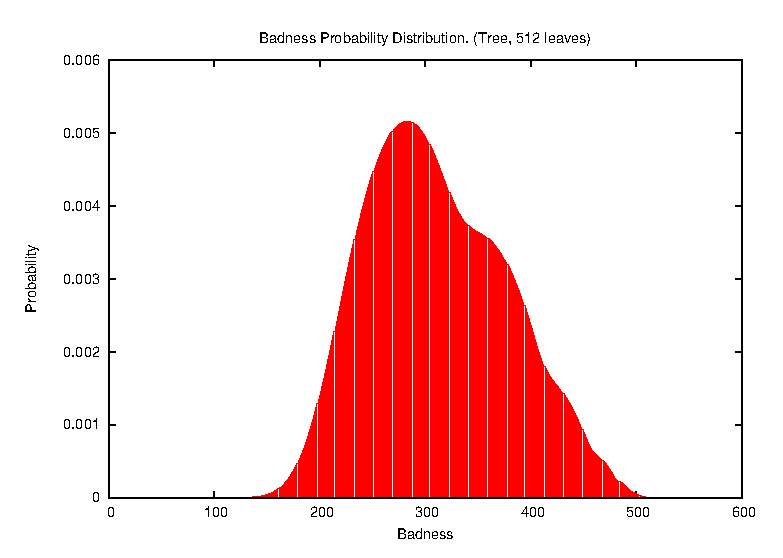
\epsfig{file=figs/badness,height=60mm}
      \caption{\label{fig:distr} Badness Probability Distribution for Binary Tree with
      512 leaves and malicious rate $\epsilon=0.1$. The mass at 512 is
      equal to 0.111111105770592 and is omitted from the graph.}
    \end{center}
  \end{figure}

  \subsection{Binary Tree with Data at all Nodes}
  \label{sec:nodes}
  Similarly to Section~\ref{sec:leaves}, let $T$ be a complete binary
  three of height $h \geq 0$. In this scenario instead of supplying data only to the
  leaves of $T$, we send a data value to any tree node. We use the
  same adversary model and define $\alpha$ to be the total number of
  tree nodes that are suppressed by the adversary: a suppressed node
  is either a malicious node, or a good node with a malicious parent.

  We can compute $P(X^k_i)$ in a similar manner:
  \begin{eqnarray}\label{eqn:notmalicious}
    P(X^k_i) &=& (1-\epsilon)\sum_{j=0}^{j=i}P(X^{k-1}_j)P(X^{k-1}_{i-j})
    \textrm{, $i<2^{k+1}-1$}\\
    P(X^k_i) &=& \epsilon \textrm{, $i=2^{k+1}-1$}\\
     P(X^0_1)&=&\epsilon,P(X^0_0)=1-\epsilon, \textrm{ and }P(X^0_i)=0
    \textrm{, $i>1$}
  \end{eqnarray}
  
  \begin{figure}[htpb!]
    \begin{center}
      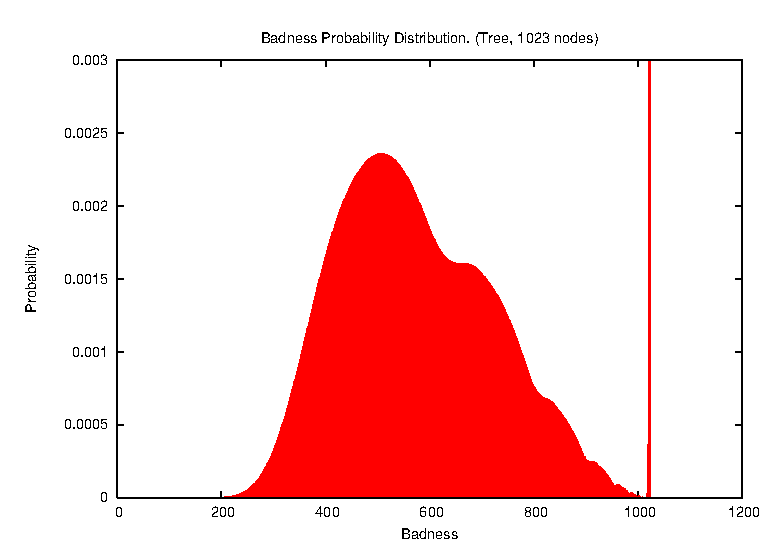
\epsfig{file=figs/badness_all,height=60mm}
      \caption{\label{fig:distr_all} Badness Probability Distribution for Binary Tree with
      1023 nodes and malicious rate $\epsilon=0.1$. The masses at 1022
      and 1023 are 0.009 and 0.1 respectively and are truncated in the
      graph.}
    \end{center}
  \end{figure}

  On Figure~\ref{fig:distr_all} we plot the probability distribution
  of a binary tree of height $9$ and malicious rate
  $\epsilon=0.1$. Similarly to the previous scenario, the graph
  exhibits some irregularities, due to the increased mass at the right
  end of the spectrum. We can intuitively explain this phenomenon
  taking into consideration that nodes closer to the root have the
  same rate of malice, but their impact increases with their
  height. This observation can justify approaches (e.g. sampling) that try to ensure
  that nodes closer to the root of the tree are malicious with smaller
  probability. 
  
  \subsection{Effect of Tree Degree}
  \label{sec:degree}
  We can extend the computation of the distribution of badness to a
  tree of degree $m$. The only differences, as compared to the binary
  case, are the different values for the boundaries ($m^h$ and
  $\frac{m^{h+1}-1}{m-1}$ instead of $2^h$ and $2^{h+1}-1$) and the
  breaking up of $i$ to $m$ sub-trees instead of two. However
  comparisons between tree aggregation structures of different degrees
  are not straightforward. For the same tree height, a ternary tree
  has significantly more nodes than a binary tree. For all practical
  purposes any comparison between aggregation structures should be done
  for trees with approximately the same number of tree nodes.

  To provide some kind of comparison among the behavior of trees of
  different degrees, we will use the expected fraction of badness as a
  basic measure.  Let $f^h_\alpha$ be the fraction of badness in a
  tree aggregation structure of height $h$. Depending on whether we
  use the approach of Section~\ref{sec:leaves} or
  Section~\ref{sec:nodes}, we can express $E[f^h_{\alpha}]$ as:\\
  
  {\bf Leaves}\\
  \begin{eqnarray}
    E[f^h_\alpha] = \epsilon + (1-\epsilon)E[f^{h-1}_\alpha]
  \end{eqnarray}

  {\bf Nodes}\\
  \begin{eqnarray}
    E[f^h_\alpha] = \epsilon + (1-\epsilon)E[f^{h-1}_\alpha]\frac{d^{h+1}-d}{d^{h+1}-1}
  \end{eqnarray}
  where $d$ is the tree degree.

  As we can see, $E[f^h_\alpha]$ is independent of the tree
  degree when we send data only to the tree leaves. When we send data
  to all tree nodes, we need to use a corrective factor to account for
  the difference in tree sizes. This corrective factor is less than
  1, and consequently the resulting expectation is smaller than the
  expectation when we send data only to the leaves (corrective factor
  of 1). This observation shows that sending data to the whole tree
  rather than to its leaves only reduces the expected fraction of
  badness. However, as the tree degree $d$ increases, the corrective
  factor becomes closer to 1 and consequently the expected fraction of
  badness increases. This phenomenon is due to the fact that as tree
  degree increases, the fraction of the leaves compared to the total
  number of tree nodes increases. Therefore, we can say that the
  expected fraction of badness sending data to the leaves only is an
  upper bound of the expected fraction of badness regardless of the
  method of dissemination. 


  %Using the observations from the previous paragraph, we can conclude
  %that using a binary aggregation tree in which we send data to all
  %tree nodes results in the smallest average fraction of badness. {\bf
  %It will be excellent if we can show that minimizing the expected
  %average fraction of badness will also minimize the other badness
  %moments, so that we can reason about the cases when we have
  %replication $c > 1$. But tests show that this is not the case}

  On Figure~\ref{fig:exp_badness} we plot the expected fraction of
  badness for trees of increasing height. We observe that as the tree
  height increases the expected fraction of badness increases as
  well. We can use this graph to reason about the security
  characteristics of trees of different degrees. Let $T_1$ and $T_2$
  be two complete trees with approximately the same number of nodes
  with degrees $d_1 < d_2$ and heights $h_1 > h_2$. Since $h_1 >
  h_2$, $E[f^{h_1}_{\alpha}] > E[f^{h_2}_{\alpha}]$. These
  inequalities show that the higher the tree degree, the smaller the expected level of
  badness. Consequently to minimize the expected level of badness, it
  is desirable to build trees of higher degrees. However, the higher
  the tree degree, the higher, the workload for an individual
  aggregator. Moreover, trees of higher degrees are harder to
  maintain in a distributed environment. 

  \begin{figure}[htpb!]
    \begin{center}
      \epsfig{file=figs/expfrac.eps,height=60mm}
      \caption{\label{fig:exp_badness} Expected fraction of badness as a
      function of tree height.}
    \end{center}
  \end{figure}

  \subsection{Probability of Suppression}
  \label{sec:supress}
  We study the probability that no copy of a single value $v$ sent $c$ times to
  randomly chosen (with replacement) tree nodes is reported by the
  root of the tree. We will refer to this probability as the
  \emph{probability of suppression}. Let $A$ be the event that all $c$
  copies of $v$ are suppressed. Let $f_\alpha$ be the ratio of the
  level of badness to the total number of tree leaves
  (Section~\ref{sec:leaves}) or the total number of tree nodes
  (Section~\ref{sec:nodes}). Defined in this way $f_\alpha$ is equal
  to the probability that a single copy of $v$ is
  suppressed. Therefore, $P(A|\alpha)=f_{\alpha}^c$ and:
  \begin{eqnarray}
    P(A) = \sum_{\alpha=0}^{\alpha_{max}}f_{\alpha}^cP(\alpha)
  \end{eqnarray}
  where $\alpha_{max}$ is the maximum possible badness ($2^h$ for
  Section~\ref{sec:leaves}, and $2^{h+1}-1$ for Section~\ref{sec:nodes}).
  When $c=1$, we have that $P(A)=E[f_{\alpha}]$.

  \subsection{Effect of Tree Height}
  \label{sec:height}
  As tree height increases, the expected fraction of badness
  increases (Section~\ref{sec:degree}). We used this observation to
  justify the design decision of trying to construct shorter trees by
  increasing their degree. We can further decrease the expected
  fraction of badness by using multiple trees of smaller height. If
  the querier is willing to perform some additional amount of work, we
  can organize the existing aggregator nodes into multiple shorter
  trees and partition the data to be aggregated. The expected fraction
  of badness will be at most the expected fraction of badness of the
  tallest constructed tree.

  On Figure~\ref{fig:multiple_trees} we plot the expected fraction of
  badness for a scenario in which there are 4095 total aggregators
  with rate of malice $\epsilon=0.1$. 

  \begin{figure}[htpb!]
    \begin{center}
      \epsfig{file=figs/multiple_trees,height=60mm}
      \caption{\label{sec:multiple_trees} Expected Fraction of Badness
      a Function of the Number of Aggregation Trees. Total number of
      aggregators 4095, $\epsilon=0.1$.}
    \end{center}
  \end{figure}

  \subsection{Effect of Replication}
  \label{sec:replicate}
  In Section~\ref{sec:supress} we derived a formula for the
  probability of suppression of a single value that is sent $c$ times
  to the aggregation structure. By increasing $c$, this probaility
  decreases, ands its complement (the probability of at least one copy
  not beight surpressed) increases. On Figure~\ref{fig:pb} we plot the
  complementary probability. we observe that 

  \begin{figure}[htpb!]
    \begin{center}
      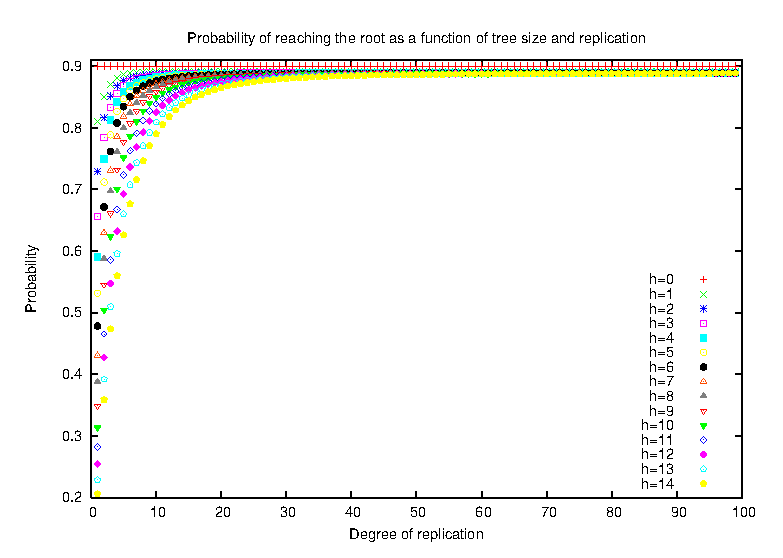
\epsfig{file=figs/tree_size,width=90mm}
      \caption{\label{fig:pb} Probability of at least one copy not
      being suppressed as a function of tree size and degree of
      replication. Rate of malice, $\epsilon=0.1$}
    \end{center}
  \end{figure}
  

  
  
%%   \section{Leaves vs. Nodes}
  
%%   where the initial factor of $(1-\epsilon)$ accounts for the fact
%%   that the root of the tree is not malicious.

%%   When $i=2^k$, the root will be malicious with probability $\epsilon$
%%   and not malicious with probability $(1-\epsilon)$. This case
%%   adds a small modification to Equation~\ref{eqn:notmalicious}:
%%   \begin{eqnarray}
%%     P(X^k_i) = \epsilon +
%%     (1-\epsilon)\sum_{j=0}^{j=i}P(X^{k-1}_j)P(X^{k-1}_{i-j})
%%     \textrm{, $i=2^k$} 
%%   \end{eqnarray}
%%   Finally, to terminate the recursive definition we have:
%%   \begin{eqnarray}
%%     P(X^0_1)=\epsilon,P(X^0_0)=1-\epsilon, \textrm{ and }P(X^0_i)=0
%%     \textrm{, $i>1$}
%%   \end{eqnarray}

%%   \begin{eqnarray}
%%     P(A) = \sum_{\alpha=0}^{\alpha=2^h}f_\alpha P(X^h_\alpha)
%%   \end{eqnarray}


%%   We can use $\alpha$ to estimate the probability that a value $v$ sent
%%   $c$ times to tree leaves chosen at random with replacement will be
%%   reported by the root of the tree. Let $A$ be the event that a single
%%   copy of $v$ does not get reported by the root. We have that $A$ occurs if and
%%   only if $v$ is sent to a suppressed leaf. Let $f_\alpha$ be the
%%   fraction of subverted leaves. We have that $P(A|\alpha)=f_\alpha$ and
%%   $P(\overline{A}|\alpha)=1-f_\alpha$. 

%%   Using the probability distribution, we can compute $P(A)$. We can
%%   even generalize to situations in which we send $c \geq 1$ copies of
%%   a value. Let $B$ be the event that when we send $c$ copies
%%   of the value to leaves chosen at random with replacement
%%   one of the copies is reported by the root. Clearly, $P(B|\alpha) =
%%   1-f_\alpha^c$ and therefore:
%%   \begin{eqnarray}
%%     P(B)=\sum_{\alpha=0}^{\alpha=2^h}(1-f_\alpha^c)P(X^h_\alpha)
%%   \end{eqnarray}


%%   On Figure~\ref{fig:pb} we plot $P(B)$ as a function of the
%%   aggregation tree size and the degree of replication. We observe that
%%   as the aggregation tree size increases, $P(B)$ decreases for the
%%   same values of $c$. This graph demonstrates an interesting property
%%   of aggregation trees: as the tree becomes taller, the probability of
%%   of data being suppressed increases. This is both a useful and
%%   intuitive observation: hierarchical aggregation increases the
%%   probability of suppression. We can exploit this fact to control the
%%   probability of suppression. If a querier is willing to do some part
%%   of the aggregation itself, then we can partition data among multiple smaller
%%   aggregation trees and decrease the probability of suppression.
  \subsection{Aggregation Bounds}
  
  {\bf Probability that a Min/Max is $k$ Positions Away from the
  Correct Min.}
  Let $X$ be a random variable describing the distance of the reported
  smallest/largest element from the true smallest/largest element. For
  a given level of badness, we have: $P(X=k|\alpha) = (f_{\alpha}^c)^k(1-f_{\alpha}^c)$. Accounting for all
  possible levels of badness:
  \begin{eqnarray}
    P(X=k)=\sum_{\alpha=0}^{2^h}(f_{\alpha}^c)^k(1-f_{\alpha}^c)P(\alpha)
  \end{eqnarray}
  For the expectation of $X$ we have:
  \begin{eqnarray}
    E[X] = \sum_{k=0}^{n-1}k\sum_{\alpha=0}^{2^h}(f_{\alpha}^c)^k(1-f_{\alpha}^c)P(\alpha)
  \end{eqnarray}
  where $n$ is the number of distinct elements.
%  When we condition by $\alpha$, $X$ has a modified geometric
%  distribution and $E[X|\alpha] =
%  \frac{f_{\alpha}^c}{1-f_{\alpha}^c}$. Therefore:  
%  \begin{eqnarray}
%    E[X] = \sum_{\alpha=0}^{\alpha=2^h}\frac{f_{\alpha}^c}{1-f_{\alpha}^c}P(\alpha)
%  \end{eqnarray}
%
%  {\bf Note:} This is not exactly the case: k does not go to infinity.
  
  {\bf Note:} While we can argue about the distance of the reported
  extreme value, it is impossible to argue about its difference in
  magnitude with respect to the actual extreme. Such analysis requires
  knowledge of the actual distribution of the data values.

  {\bf Probability that an FM zero position is $k$ smaller than the
  actual position.} A single FM bitvector has a structure similar to the one
  shown of Figure~\ref{fig:bitvector}. FM uses the position of the
  least significant zero bit to compute its estimate. An adversary can
  only decrease this position (See protection against increase (coming
  soon)). Let $l$ be the correct position of the least significant
  zero bit and $X$ be a random variable describing the position of the
  least significant zero. For $X$ to be equal to $k$ ($0\leq k \leq l$), all
  bits prior to $k$ need to be turned on. For each bit position smaller than $k$ there is at least one data
  value that turns on this bit, and on the average, if the bit's
  position is $i$, there are $2^{l-i}$ such values. We have:
  \begin{eqnarray}
    P(X=k) \geq \sum_{\alpha=0}^{2^h}(1-f_{\alpha}^c)^{k-1}P(\alpha)
  \end{eqnarray}

  For the expectation of $X$, we have:
  \begin{eqnarray}
    E[X] \geq \sum_{k=0}^{\log_2{n}}k\sum_{\alpha=0}^{2^h}(1-f_{\alpha}^c)^{k-1}P(\alpha)
  \end{eqnarray}






\section{Probability}

  We examine the problem of Butterfly network
  reliability. Let $B$ be a butterfly network of degree 2 with $n$
  nodes total, such that all are present on each level.  We label the
  levels of $B$ staring from 0 to $\log_2n$, where 0 is the input
  level. The basic property of the  so defined Butterfly network is
  that any of its inputs is eventually propagated 
  to all network nodes. Let's assume that each input is initially provided
  to $c \geq 1$ independently chosen random nodes on level 0. We will
  study the probability that a Butterfly node on a given level
  receives a particular input.

  {\bf No Failures.} Assume that no node of $B$ fails before $B$ has
  completed its operations. Let $A$ be the event that a given node is
  the first chosen to receive a particular value on level 0. Clearly $P(A) =
  \frac{1}{n}$ and $P(\overline{A}) = \frac{n-1}{n}$. Let $B$ be the
  event that a node on level 0 was not chosen to receive a particular
  value after all $c$ trials. We have that $P(B) =
  (\frac{n-1}{n})^c$ and $P(\overline{B}) = 1-(\frac{n-1}{n})^c$.

  Let $P(k,n,c)$ be the probability that a node on level $k$ of a
  Butterfly network with $n$ nodes does not
  receive a particular value sent initially to $c$ randomly selected
  input nodes. We computed $P(0,n)$ to be $(\frac{n-1}{n})^c$. In
  general, a node $a$ does not receive value on level $k  > 0$ if $a$
  did not receive the value on level $k-1$ and if $b$ is the node $a$
  communicates with on level $k$, then $b$ also did not receive the
  value on level $k-1$. We can express this probability as: 

  \begin{eqnarray*}
    P(k,n,c) = P(k-1,n,c)P(k-1, n-2^{k-1},c)
  \end{eqnarray*}
  Where the first factor is the probability that $a$ did not receive
  the value, and the second factor is the probability that $b$ did not
  receive the value.

  For $k =1$, we have that:
  \begin{eqnarray*}
    P(1, n,c) &=& P(0, n,c)P(0, n-1,c) = \\
    &=&(\frac{n-1}{n})^c(\frac{n-2}{n-1})^c=\\
    &=&(\frac{n-2}{n})^c
  \end{eqnarray*}

  \begin{prop}
    $P(k,n,c) = (\frac{n-2^k}{n})^c$
  \end{prop}

  \begin{proof}
    We demonstrated that the above statement holds for $k=1$. Let
    for $k=l \leq 1$ the statement also be true. For $k=l+1$, we have:
    \begin{eqnarray*}
      P(l+1,n,c) &=& P(l,n,c)P(l, n-2^{l},c) = \\
      &=& (\frac{n-2^l}{n})^c(\frac{n-2^{l}-2^{l}}{n-2^l})^c =\\
      &=& (\frac{n-2^{l+1}}{n})^c
    \end{eqnarray*}
    $\Rightarrow P(k,n,c) = (\frac{n-2^k}{n})^c$ for any $0 \leq k
    \leq \log_2n$. 
  \end{proof}

  \begin{figure}
    \begin{center}
      \epsfig{file=figs/no_fail.eps,width=120mm}
      \caption{\footnotesize Probability of not receiving a value for
      each level of a Butterfly network with 1024 nodes, no failures, and varying
      replication factor $c$.}
      \label{test}
    \end{center}
  \end{figure}

  {\bf Independent Failures.}
  Assume that each Butterfly node can fail independently with
  probability $\epsilon$. We will compute $P(k,n,c)$ by conditioning
  on the event of a node failing. Let $A$ be the event that a node has
  not failed. We have that:
  \begin{eqnarray*}
    P(k,n,c) &=& P(k,n,c|A)P(A) +
    P(k,n,c|\overline{A})P(\overline{A})\\
    P(k,n,c|\overline{A}) &=& 1\\
    P(A) &=& 1-\epsilon\\
    P(\overline{A})&=& \epsilon      \\
    \Rightarrow P(k,n,c) &=& P(k,n,c|A)(1-\epsilon) + \epsilon
  \end{eqnarray*}
  A non failed node at level $k > 0$ does not receive a given value if
  it did not receive it at level $k-1$ and either talked to a
  non-failed node that also did not receive the value at level
  $k-1$ or talked to a failed node.Therefore:
  \begin{eqnarray*}
    P(k,n,c|A) &=& P(k-1,n,c|A)(\epsilon +\\
    &&(1-\epsilon)P(k-1,n-2^{k-1},c*|A))
  \end{eqnarray*}
  where $P(k-1,n-2^{k-1},c*|A)$ is the probability that the other good
  node did not receive the given value. We use $c*$ to denote the fact
  that it is unclear what value of $c$ should be used. Let $P'(k, n,
  c)$ be the probability that two non-failed nodes that communicate on level
  $k$ have not received a given value. Let also $P(B_i^k)$ be the
  probability that in the initial distribution of the given value,
  there have been $i$ selections in the first $2^k$ Butterfly
  nodes. We have:
  \begin{eqnarray*}
    P'(k, n, c) = \sum_{i=0}^{i=c}P(k-1,2^{k-1},i|A)P(k-1, n-2^{k-1}, c-i|A)P(B_i^{k-1})
  \end{eqnarray*}

  Let $X_{n,c}^k$ be a random variable describing the number of
  selections in the first $2^k$ nodes of a network of $n$ total nodes
  and replication factor $c$. We have that:
  \begin{eqnarray*}
    P(X_{n,c}^0=i) = {c \choose i}(\frac{1}{n})^i(\frac{n-1}{n})^{c-i} 
  \end{eqnarray*}
  We can define $P(X_{n,c}^k=i)$ recursively as:
  \begin{eqnarray*}
    P(X_{n,c}^k=i) = \sum_{j=0}^{j=i}P(X_{n,c}^{k-1}=
    i-j)P(X_{n-2^{k-1},c-i+j}^{k-1}= j)
  \end{eqnarray*}

  \noindent Therefore:
  \begin{eqnarray*}
    P(k,n,c|A) = \epsilon P(k-1,n,c|A) + (1-\epsilon)P'(k,n,c)
  \end{eqnarray*}
   
  \begin{figure}
    \begin{center}
      \epsfig{file=figs/with_fail_0_1.eps,width=120mm}
      \caption{\footnotesize Probability that a non-failed node will
      not receive a value for each level of a Butterfly network with
      1024 nodes, 0.1 failure rate, and varying replication factor $c$.}
      \label{test}
    \end{center}
  \end{figure}

  \begin{figure}
    \begin{center}
      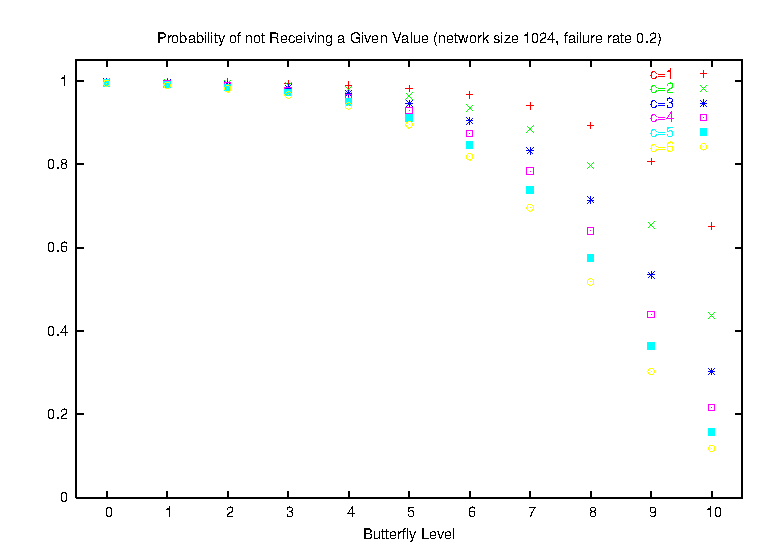
\epsfig{file=figs/with_fail_0_2.eps,width=120mm}
      \caption{\footnotesize Probability that a non-failed node will
      not receive a value for each level of a Butterfly network with
      1024 nodes, 0.2 failure rate, and varying replication factor $c$.}
      \label{test}
    \end{center}
  \end{figure}

  





\section {Binary Tree Network Reliability}

  We examine the problem of binary tree network reliability. Let $B$
  be a complete binary tree with $n$ leaf nodes and $\log_2{n}+1$
  levels. We label the levels of $B$ staring from 0 to $\log_2n$, where 0 is the leaf
  level. Let $v$ be a value we would like to send to the root of the
  tree by sending it to $c \geq 1$ leaf tree nodes. Let $P(k,n,c)$ be
  the probability that a node at level $k$ in a binary tree with $n$
  leaves will not receive $v$ when we initially send $c$ copies of it
  to leaf tree nodes chosen uniformly at random with replacement.

  {\bf No failures}
  Assume that no node of $B$ fails before $B$ has completed all
  forwarding. Let $A$ be the event that a leaf node is selected to
  receive a copy of $v$ after the first selection: $P(A) =
  \frac{1}{n}$ and $P(\overline{A}) = \frac{n-1}{n}$. Let $B$ be the
  event that a leaf node is not selected to receive a copy of $v$
  after $c$ selections: $P(B) = (\frac{n-1}{n})^c$. 

  \noindent $\Rightarrow P(0,n,c)= (\frac{n-1}{n})^c$.
  A tree node on level k, will not receive a copy of $v$ if none of
  its children on level $k-1$ have received a copy. Therefore:
  \begin{eqnarray*}
    P(k,n,c) = P(k-1,n,c)P(k-1, n-2^{k-1},c)
  \end{eqnarray*}
  Where the first factor is the probability that $a$ did not receive
  the value, and the second factor is the probability that $b$ did not
  receive the value.

  For $k =1$, we have that:
  \begin{eqnarray*}
    P(1, n,c) &=& P(0, n,c)P(0, n-1,c) = \\
    &=&(\frac{n-1}{n})^c(\frac{n-2}{n-1})^c=\\
    &=&(\frac{n-2}{n})^c
  \end{eqnarray*}

  \begin{prop}
    $P(k,n,c) = (\frac{n-2^k}{n})^c$
  \end{prop}

  \begin{proof}
    We demonstrated that the above statement holds for $k=1$. Let
    for $k=l \leq 1$ the statement also be true. For $k=l+1$, we have:
    \begin{eqnarray*}
      P(l+1,n,c) &=& P(l,n,c)P(l, n-2^{l},c) = \\
      &=& (\frac{n-2^l}{n})^c(\frac{n-2^{l}-2^{l}}{n-2^l})^c =\\
      &=& (\frac{n-2^{l+1}}{n})^c
    \end{eqnarray*}
    $\Rightarrow P(k,n,c) = (\frac{n-2^k}{n})^c$ for any $0 \leq k
    \leq \log_2n$. 
  \end{proof}

  {\bf Independent Failures} Assume that each tree node can fail
  independently with probability $\epsilon$. A node at level $k$ fails
  with probability $\epsilon$ and  does not fail with probability
  $1-\epsilon$. A failed node does not receive $v$ with probability
  $1$. Therefore:
  \begin{eqnarray*}
    P(k,n,c) = \epsilon + (1-\epsilon)P'(k-1, n, c)
  \end{eqnarray*}
  where $P'(k-1,n,c)$ is the joint probability that both children of
  the node do not receive a copy of $v$.

  Let $P(B_i^k)$ be the probability that in the initial distribution
  of $v$, there have been $i$ selections in the first $2^k$ tree leaf
  nodes. We can express $P'(k,n,c)$ as:
  \begin{eqnarray*}
    P'(k, n, c) = \sum_{i=0}^{i=c}P(k-1,2^{k-1},i)P(k-1, n-2^{k-1}, c-i)P(B_i^{k-1})
  \end{eqnarray*}

  Let $X_{n,c}^k$ be a random variable describing the number of
  selections in the first $2^k$ nodes of a network of $n$ total nodes
  and replication factor $c$. We have that:
  \begin{eqnarray*}
    P(X_{n,c}^0=i) = {c \choose i}(\frac{1}{n})^i(\frac{n-1}{n})^{c-i} 
  \end{eqnarray*}
  We can define $P(X_{n,c}^k=i)$ recursively as:
  \begin{eqnarray*}
    P(X_{n,c}^k=i) = \sum_{j=0}^{j=i}P(X_{n,c}^{k-1}=
    i-j)P(X_{n-2^{k-1},c-i+j}^{k-1}= j)
  \end{eqnarray*}



\section{Absorbed Documents}

problem.tex



\end{document}

